\documentclass[a4paper,
               11pt,
               parskip=half,
               headinclude,
               titlepage=false]{scrartcl}

%%%%%%%%%%%%%%%%%%%%%%%%%%%%%%%%%%%%%%%%
\newcommand{\metaauthor}{moPsy}
\newcommand{\metatitle}{Eurorack Power Breakout User Manual}
\newcommand{\metarev}{1.1}
%%%%%%%%%%%%%%%%%%%%%%%%%%%%%%%%%%%%%%%%


\usepackage[utf8]{inputenc}

\usepackage[T1]{fontenc}        % Tries to use Postscript Type 1 Fonts for better rendering
\usepackage{lmodern}            % Provides the Latin Modern Font which offers more glyphs than the default Computer Modern
\usepackage[sfdefault]{carlito}
\usepackage[intlimits]{amsmath} % Provides all mathematical commands
\usepackage[protrusion=true,
            expansion,
            kerning=true,
            babel=true]{microtype}
\usepackage{fontawesome}

\usepackage[english]{babel}
\usepackage[english]{isodate}

\usepackage{eurosym}
\usepackage[shortlabels]{enumitem}

\usepackage{grffile}            % Allow you to include images (like graphicx). Usage: \includegraphics{path/to/file}

\usepackage[ugly]{units}        % Allows you to type units with correct spacing and font style. Usage: $\unit[100]{m}$ or $\unitfrac[100]{m}{s}$

\usepackage{xspace}             % Use \xpsace in macros to automatically insert space based on context. Usage: \newcommand{\es}{ESPResSo\xspace}
\usepackage[dvipsnames,table]{xcolor}             % Obviously colors. Usage: \color{red} Red text
\usepackage{booktabs}           % Nice rules for tables. Usage \begin{tabular}\toprule ... \midrule ... \bottomrule


%\usepackage[hang]{subfigure}  % unterteilte Abbildungen
\usepackage{setspace}          %fuer dem Zeilanabstand
\usepackage[hang,bf,footnotesize]{caption}   % bessere Bildunterschriften
\usepackage{wrapfig}

\usepackage{csquotes}


\usepackage[hyphens]{url}                % Lets you typeset urls. Usage: \url{http://...}
\usepackage[pdftex,colorlinks=true,linkcolor=black,citecolor=black,urlcolor=black]{hyperref}
\hypersetup{
  pdftitle    = {\metatitle},
  pdfsubject  = {Assembly Guide},
  pdfauthor   = {\metaauthor},
  pdfkeywords = {} ,
  pdfcreator  = {pdflatex},
  pdfproducer = {LaTeX with hyperref}
}
%%%%%%%%%%%%%%%%%%%%%%%%%%%%%%%%%%%%%%%%

\usepackage{pdfpages}

\usepackage{tabularx}


\usepackage[headsepline, footsepline]{scrlayer-scrpage}
\setlength{\headheight}{34pt} % logo height
\clearpairofpagestyles
\ohead{
\vfill%
\begin{tabular}{@{}l l@{}}

\includegraphics[height=2em]{moPsy_logo}\hspace*{-0.1cm}
\end{tabular}
}
\ihead{
\vfill%
{\huge Eurorack Power Breakout} \,v\metarev\, User Manual%
}
\ofoot{Page \thepage}
\setkomafont{pageheadfoot}{\sffamily\footnotesize}
\setkomafont{pagination}{}
\pagestyle{scrheadings}


%\usepackage{background}

%\usepackage[section]{placeins} % keep figures in their section


\definecolor{level_easy}{rgb}{0.2, 0.6, 0.1}

\definecolor{row1}{rgb}{1.0, 1.0, 1.0}
\definecolor{row2}{rgb}{0.93, 0.93, 0.99}



\begin{document}


\begin{minipage}[b]{10.5cm}
\setlength{\parskip}{\medskipamount}
\section*{Thank you for choosing a 
\includegraphics[height=0.8em]{moPsy_logo} product!}

This manual provides information on the \textbf{Eurorack Power Breakout} board.
We hope that all questions will be answered.
If you encounter a problem or have further questions,
please do not hesitate and reach out to us at \href{mailto:contact@mopsy-music.de}{\texttt{contact@mopsy-music.de}}.


%\vspace{1em}
\begin{center}
Enjoy! \quad 
\includegraphics[height=0.8em]{peace_love_music}
\end{center}

\end{minipage}%
\hspace{0.5cm}
\begin{minipage}[]{4cm}
\vspace{-3cm}
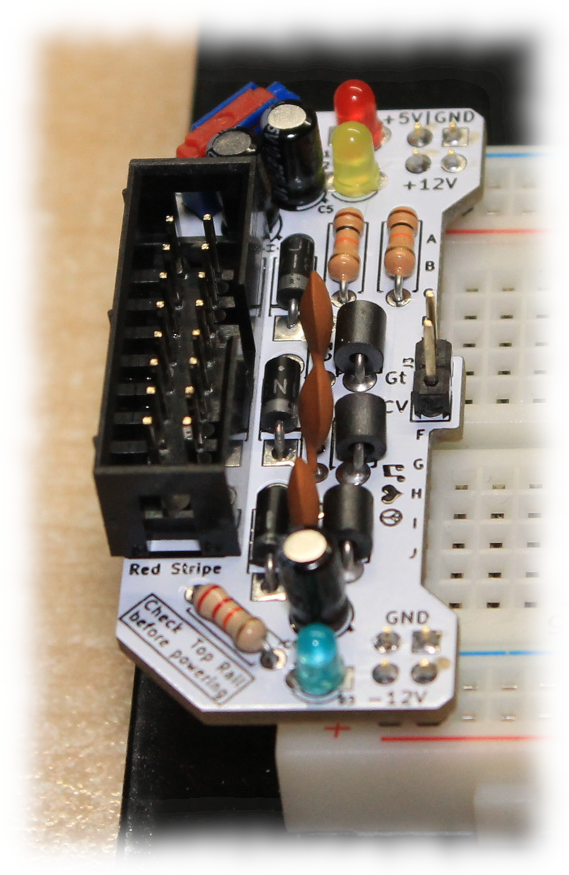
\includegraphics[width=4cm]{eurorack-power-breakout-frame}
\end{minipage}

\vspace{-3em}
\section*{About the Eurorack Power Breakout board}

The \textbf{Eurorack Power Breakout} board provides the Eurorack power bus on a breadboard.
It allows for a \textbf{quick setup} of power supply components, so that you can immediately start prototyping.

The \textbf{main features} are:
\begin{itemize}[noitemsep]
 \item Reverse polarity protection diodes
 \item Basic filtering on the power supply lines
 \item Selection for 5V/GND on one of the power rails
 \item Breakout for CV and Gate signals from the extended bus
\end{itemize}


\section*{Installation}

Install the breakout board on your breadboard power rails as shown in the picture above.
If your board has color markings,
it is beneficial to align the \unit[+12]V/\unit[-12]V pins with the red lines.

To \textbf{connect power} …
\begin{enumerate}[noitemsep]
 \item Please make sure that your cabinet is \textbf{disconnected from the mains} and has no power.
 \item The board is connected with a \textbf{16-pin} (2x8) bus cable.
 \item \textbf{Check your power cable and the polarity.} The coloured (\textbf{\color{red}red}) line on the cable (pin~1) needs to be connected to the \textbf{\unit[-12]{V}} rail.
 \item If you plug the board backwards, it may burn out.
 Unfortunately this cannot be covered by the warranty.
\end{enumerate}

The board itself draws a maximum of \textbf{\unit[2]mA} from each rail.


\begin{minipage}[]{10.5cm}
\setlength{\parskip}{\medskipamount}
\section*{Setup and Use}

The first step on each use is to set up the \textbf{\color{red}Voltage Selector} (1), which allows you to change the top rail between \textbf{\unit[+5]V} and \textbf{GND} by placing the jumper in the respective position. Do not bridge the outer pins, as this will short your power supply!

Please take extra care of this jumper, as a \textbf{wrong setting may destroy your components!}

%Hence the warning:

\begin{center}

\includegraphics[height=3em]{check-power-rail-warning}
\end{center}

The \textbf{LEDs} on the board will light up according to selected the voltages,
\textbf{\color{red}RED} for \unit[+5]V, \textbf{\color{orange!80}YELLOW} for \unit[+12]V and \textbf{\color{blue}BLUE} for \unit[-12]V.

\end{minipage}%
\hspace{0.5cm}
\begin{minipage}[]{4cm}
\vspace{-1cm}
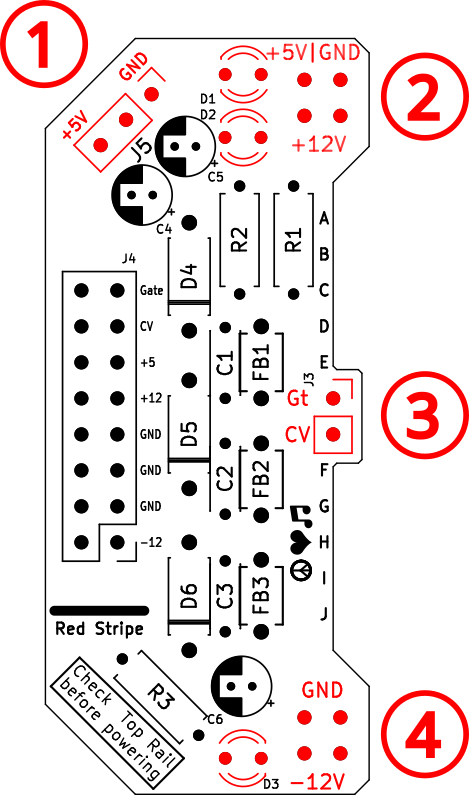
\includegraphics[width=4cm]{eurorack-power-breakout-labels}
\end{minipage}

\vspace{2em}

The board provides the \textbf{Eurorack power lines} on your breadboard power strips with the following configuration:
\begin{itemize}
 \item The \textbf{TOP line} (2) presents \textbf{\color{red}\unit[+5]V} or \textbf{\color{red}GND}, depending on the jumper (1), and \textbf{\color{red}\unit[+12]V}.
 \item The \textbf{BOTTOM line} (4) presents \textbf{\color{red}GND} and \textbf{\color{red}\unit[+12]V}.
\end{itemize}

If there are markings on the breadboard, the labels should align.


\vspace{2em}

The \textbf{MIDDLE line} (3) presents \textbf{\color{red}Bus Gate} and \textbf{\color{red}Bus CV}.

Please note that the \textbf{input/output configuration} of these signals depends on your application and is not influenced by the breakout board.


\section*{Online Resources}

More about the board  …
\begin{itemize}[noitemsep]
 \item on my website: \url{https://www.mopsy-music.de/tools/eurorackpowerbreakout}
 \item on GitHub: \url{https://github.com/moPsy-project/eurorack-power-breakout}
 \item via e-mail: \href{mailto:contact@mopsy-music.de}{\texttt{contact@mopsy-music.de}}
\end{itemize}


\end{document}
